%7 делится на две главы. Задача с чертежом коорд.оси (предвор сведения, разработанные библ функции, шаблоны)
% вторая - задача на сравнение чисел (как устроено округление,autoLateX )
\section{Задачи №7 ОГЭ (сравнение чисел)}
В проекте присутствует отдельный шаблон, посвящённый задачам на сравнение действительных чисел. 
Основная цель подобных заданий --- научить учащегося ориентироваться в числовой прямой, дробях и приближённых значениях корней.  

Так как в задачах встречаются как обыкновенные дроби, так и десятичные приближения квадратных корней, 
важно уметь корректно округлять результаты. Для этого используется метод \verb|toFixed(1)|, позволяющий оставить одно десятичное число. Например:

\begin{lstlisting}[language=JavaScript]
let correctVal = ((frac1 + frac2) / 2);
let correct = correctVal.toFixed(1).ts();
\end{lstlisting}
Здесь мы берём среднее значение между двумя дробями, а затем округляем его до одного знака после запятой, 
чтобы получить корректный ответ, который предлагается ученику.  
Пример:
\lstinputlisting[]{code/7/205843.js} 
До:
После:
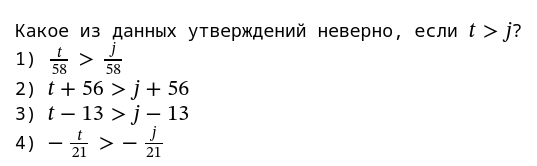
\includegraphics[width=1\textwidth]{205843-7-3.png}
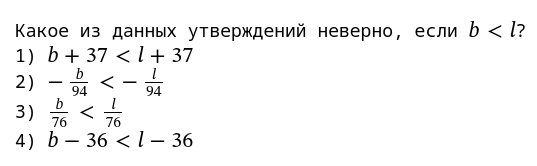
\includegraphics[width=1\textwidth]{205843-7-2.png}
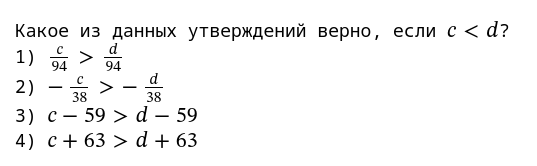
\includegraphics[width=1\textwidth]{205843-7-1.png}

Для проверки знаний учащегося необходимо не только предъявить правильный ответ, 
но и сформировать несколько правдоподобных «ловушек». 
В нашем проекте это реализовано через генерацию трёх ложных ответов. 
Ложные варианты создаются с помощью небольших шумов (\verb|noise|), добавляемых к правильному значению.  

\begin{lstlisting}[language=JavaScript]
let wrong = new Set();
while (wrong.size < 3) {
    let noise = slKrome([0], -7, 7) * 0.1;
    let candidate = +(correctVal + noise).toFixed(1);

    if (candidate <= 0 || candidate > frac1 && candidate < frac2 
        || candidate === +correctVal.toFixed(1)) {
        continue;
    };
    wrong.add(candidate.ts());
}
\end{lstlisting}

Таким образом, в итоговом задании всегда предлагается \textbf{4 варианта ответа}: один правильный и три ложных.  

После задания параметров задачи и вариантов ответа вызывается функция \verb|AtoB(3)|. 
Она отвечает за автоматическую генерацию списка вариантов с правильным ответом, расположенным случайным образом.  

\begin{lstlisting}[language=JavaScript]
NAtask.setTask({
    text: 'Какое из следующих чисел заключено между числами ${' + text1 + '}$ и ${' + text2 + '}$?',
    answers: correct,
    wrongAnswers: Array.from(wrong)
});

AtoB(3, { autoLaTeX: true });
\end{lstlisting}

Чтобы не окружать каждую формулу знаками \verb|$...$|, используется параметр \verb|{ autoLaTeX: true }|. 
Это позволяет сразу включать математические выражения (например, дроби и корни) прямо в текст задачи. 
В результате формулы корректно отображаются в интерфейсе без дополнительной ручной разметки.  

В результате ученик видит задачу: 
\textit{«Какое из следующих чисел заключено между числами …?»}, 
к которой автоматически предлагаются четыре варианта ответа.  
% расфосовать задачи чуть более аккуратно и с фотографиями до /после
Пример:

\lstinputlisting[]{code/7/311420.js} 
До:
После:
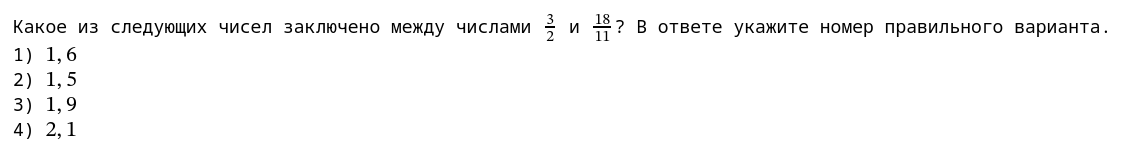
\includegraphics[width=1\textwidth]{311420-7-1.png}
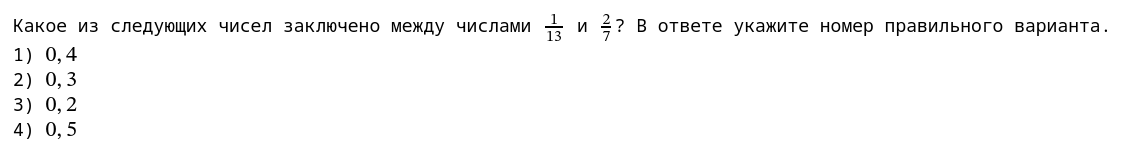
\includegraphics[width=1\textwidth]{311420-7-2.png}

\lstinputlisting[]{code/7/317132.js} 
До:
После:
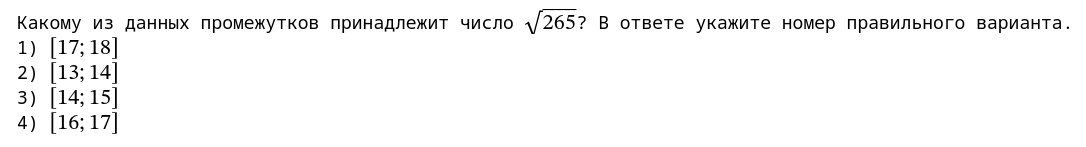
\includegraphics[width=1\textwidth]{317132-7-1.png}
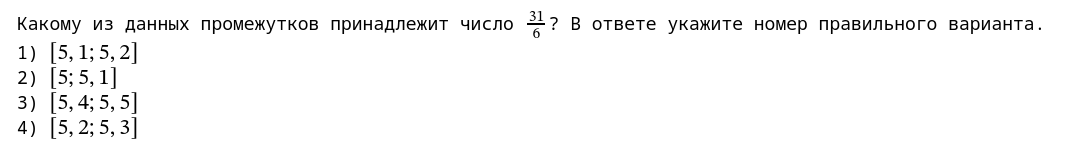
\includegraphics[width=1\textwidth]{317132-7-2.png}

Исходная задача:
Сгенрированная задача:


%\begin{figure}[h]
%\center{\includegraphics[width=1\linewidth]{image}}
%\caption{Зависимость сигнала от шума для данных.}
%\label{ris:image}
%\end{figure}


На рис.~\ref{ris:317132} представлены исходная и сгенерированные задачи по шаблону №317132.


\begin{figure}[h]
\begin{minipage}[h]{0.95\linewidth}
\center{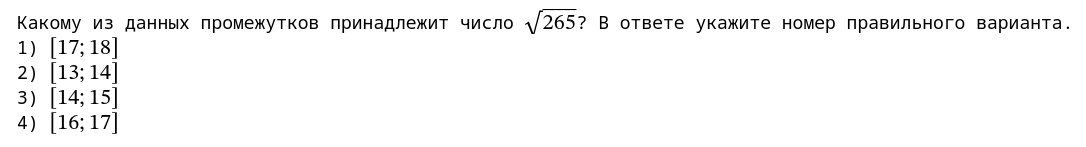
\includegraphics[width=1\linewidth]{317132-7-1.png}} \\а)
\end{minipage}
\vfill
\begin{minipage}[h]{0.95\linewidth}
\center{%
    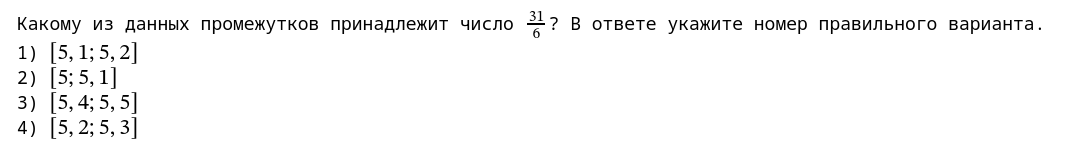
\includegraphics[width=1\linewidth]{317132-7-2.png}
    \\
    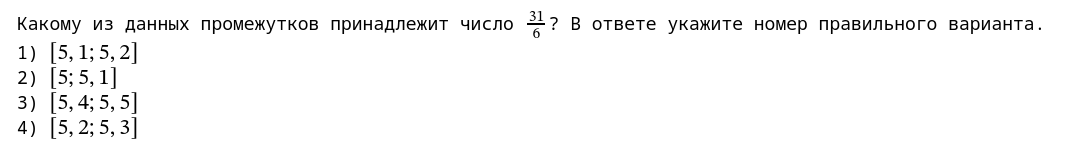
\includegraphics[width=1\linewidth]{317132-7-2.png}
} б) \\
\end{minipage}
\caption{Задачи, соответствующие шаблону 317132:
\\
а) исходная; б) сгенерированные}
\label{ris:317132}
\end{figure}


%%%%%%
%%%%%%

Ура?